%%Roll no: 130010042, Name: Shobhit Voleti

\documentclass[11pt]{article}
\usepackage{amsmath}
\usepackage{amssymb}
\usepackage{amsthm}
\usepackage{graphicx}
\usepackage{float}
\usepackage{hyperref}


\newtheorem*{defn}{Definition}

\title{Analysis of Pendulum with Friction}
\author{Shobhit Voleti 130010042 \thanks{This document has been prepared as part of the requirements for the first course project}}
\date{\today}

\begin{document}
\maketitle
\begin{abstract}
\centering{Github Repository: \href{https://github.com/shobhitvoleti/frictionpendulum}{\textbf{Friction Pendulum}}}
\newline This document gives brief introduction to the not so simple pendulum with friction. A comprehensive analysis of the system substantiated by appropriate simulation results have been presented.
\end{abstract}
\section{Introduction \cite{google}}
An extension to the analysis of a simple pendulum, analysis of a pendulum with friction involves dealing with terms that arise due to friction encountered during the angular motion of the pendulum.

This consists of a point mass attached to an inextensible string. A force acting on the point mass is its weight. The weight can be split into two components: the tangential force and the force acting away from the center of rotation. The latter force, shown in brown, is balanced by the reaction force acting towards the center and so can be ignored.


\newpage
\section{Dynamics \cite{nrich}}

\begin{figure}[H]
\centering
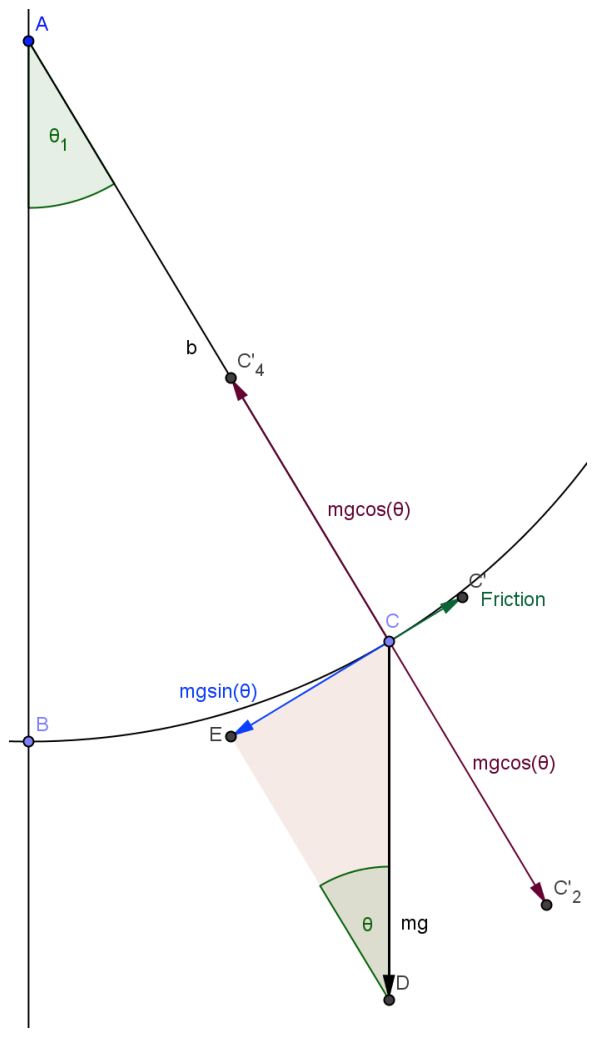
\includegraphics[width = 0.5\textwidth]{fric_pen.png}
\caption{Inverted Pendulum with sliding rod}
\label{Fig1}
\end{figure}

The force due to friction acts tangentially on the bob. Since it acts in the opposite direction to the motion, the coefficient has to be negative.

Keeping the friction coefficient constant allows the differential equation to be linear and so, easy to solve. Making the frictional force proportional to the tangential velocity v rather than to the angular velocity $\omega$ prevents the pendulum’s length from affecting the frictional force.
\hfil \break
Frictional force is given by the term,
\begin{equation} \label{eq:1}
F_s = \lambda \frac{dy}{dt}
\end{equation}

The equations that govern the motion of the system are as follows:
\begin{equation}
\label{eom}
m\ddot{y} + \lambda\dot{y} + \frac{mgy}{r}
\end{equation}

\section{Friction pendulum as generalized second order system}

General second-order system is given by :
\begin{equation}
\ddot{x} + 2\zeta\omega_0\dot{x} + \omega_0^2x = 0
\label{sec_ord_system}
\end{equation}
where $\zeta$ is called damping ratio and $\omega_0$ is called natural frequency.
\hfill \break
From \ref{eom} we can get,
\begin{equation}
\ddot{y} + \frac{\lambda}{m}\dot{y} + \frac{g}{r}y = 0
\label{pendulum}
\end{equation}

Comparing coefficient with \ref{sec_ord_system}, we get
\begin{eqnarray}
\zeta &=& \frac{\lambda}{2\sqrt{km}}, \\
\label{def_zeta}
\omega &=& \sqrt{\frac{g}{r}}
\label{def_omega}
\end{eqnarray}
\hfill \break
where,
\begin{equation}
k = \frac{mg}{r}
\label{def_k}
\end{equation}

\newpage
\section{State space model of the system\cite{google}}

We can describe the system only by its position and velocity. Therefore the state-space model
of the system is given by :

\[
\widetilde{x}=
\begin{bmatrix}
x \\
\dot{x}
\end{bmatrix}
\]

Therefore, equation of motion can be expressed as :
\[
\dot{\widetilde{y}}=
\begin{bmatrix}
y_2\\
- \frac{\lambda}{m}x_2 - \frac{k}{m}x_1 + F(y_2,y_1,t)
\end{bmatrix}
\]
\hfill \break
\section{Classification of system based on damping ratio}
\begin{itemize}
	\item{Under-damped system ($\zeta < 1$)}
	\item{Critically damped system ($\zeta = 1$)}
	\item{Over-damped system ($\zeta > 1$)}
\end{itemize}

\newpage
\noindent\textbf{Under-damped system :} \\
In under-damped system $\zeta$ is less than 1. \\
This case best describes friction encountered on most surfaces
The free response of the system is shown in the figure below.
\begin{figure}[H]
\centering
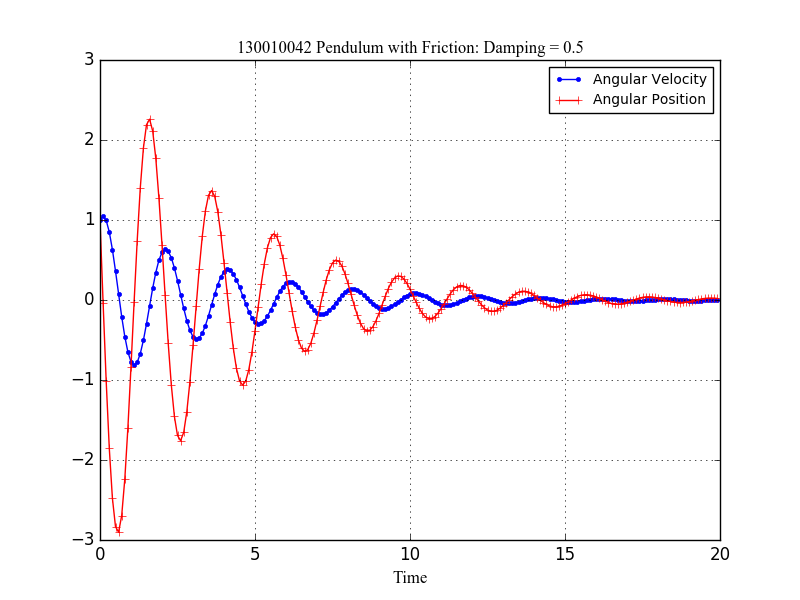
\includegraphics[width = 1.4\textwidth]{ud_pen.png}
\caption{130010042 Under-damped response}
\label{Fig2}
\end{figure}

\newpage
\noindent\textbf{Critically-damped system :} \\
In critically-damped system $\zeta$ is 1.
The free response of the system is shown in the figure below.

\begin{figure}[H]
\centering
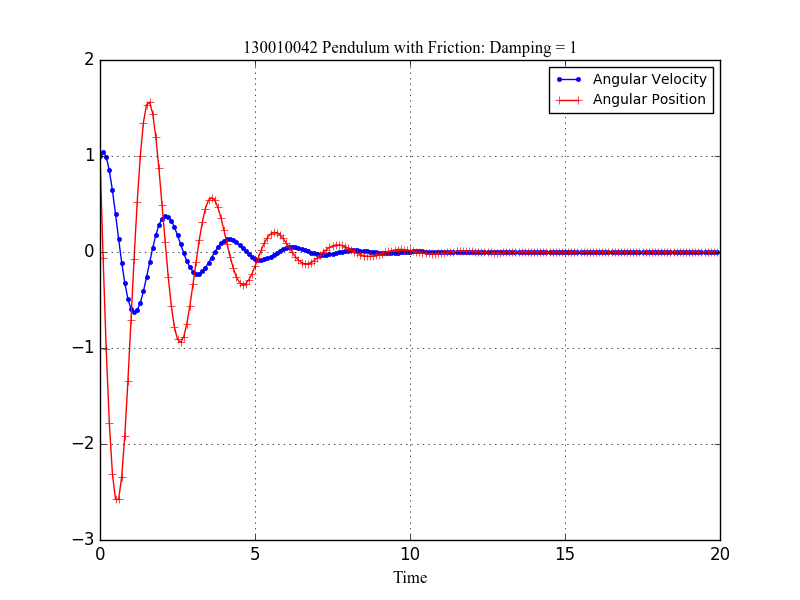
\includegraphics[width = 1.4\textwidth]{cd_pen.png}
\caption{130010042 Critically-damped response}
\label{Fig3}
\end{figure}

\newpage
\noindent\textbf{Special case :} \\
A special case of the system arises when there is zero damping i.e $\lambda = 0$ or $\zeta$ is zero. \\
The free response of the system is shown in the figure below.

\begin{figure}[H]
\centering
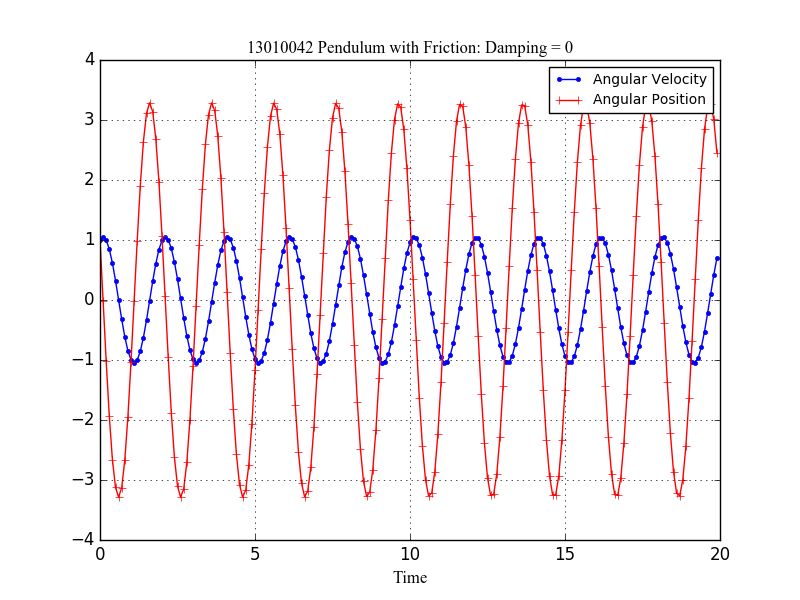
\includegraphics[width = 1.4\textwidth]{zer_pen.png}
\caption{130010042 Friction-less response}
\label{Fig4}
\end{figure}


\bibliography{bib_file}{}
\bibliographystyle{plain}

\end{document}
